% Figure for the flipbook of strategies over time

\begin{figure}
\center

	\begin{subfigure}[b]{0.4\textwidth}
	
\includegraphics[width=\linewidth]{images/findings/round2/flipbook/loser/checkpoint_000000.png}
	\caption{Starting Weights}
	\end{subfigure}
	~
	\begin{subfigure}[b]{0.4\textwidth}
	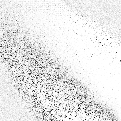
\includegraphics[width=\linewidth]{images/findings/round2/flipbook/loser/checkpoint_200000.png}
	\caption{After 200,000 games played}
	\end{subfigure}

	\begin{subfigure}[b]{0.4\textwidth}
	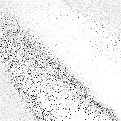
\includegraphics[width=\linewidth]{images/findings/round2/flipbook/loser/checkpoint_400000.png}
	\caption{After 400,000 games played}
	\end{subfigure}
	~
	\begin{subfigure}[b]{0.4\textwidth}
	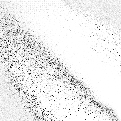
\includegraphics[width=\linewidth]{images/findings/round2/flipbook/loser/checkpoint_600000.png}
	\caption{After 600,000 games played}
	\end{subfigure}

	\begin{subfigure}[b]{0.4\textwidth}
	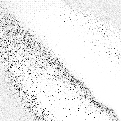
\includegraphics[width=\linewidth]{images/findings/round2/flipbook/loser/checkpoint_800000.png}
	\caption{After 800,000 games played}
	\end{subfigure}
	~
	\begin{subfigure}[b]{0.4\textwidth}
	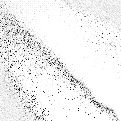
\includegraphics[width=\linewidth]{images/findings/round2/flipbook/loser/checkpoint_999999.png}
	\caption{Final Weights}
	\end{subfigure}

\caption{
	Training weights representation for a loser bracket agent's \handmaxavg\
	strategy when the agent is the dealer
	over the course of the one million games of Round 2.
}
\label{fig:r2-flip-loser}
\end{figure}
